% This is samplepaper.tex, a sample chapter demonstrating the
% LLNCS macro package for Springer Computer Science proceedings;
% Version 2.20 of 2017/10/04
%
\documentclass[runningheads]{llncs}
%
\usepackage{graphicx}
\usepackage{placeins}
\usepackage{caption}
\usepackage{subcaption}
\usepackage{amsmath}
\usepackage{hyperref}
\usepackage{xcolor}
\usepackage[linesnumbered,ruled,vlined]{algorithm2e}
\usepackage[acronym]{glossaries}

\newacronym[]{ir}{IR}{Infra Red}
\newacronym[]{fov}{FOV}{Field of View}
\newacronym[]{pdf}{PDF}{Probability Density Function}
\newacronym[]{irr}{IRR}{Infinite Impulse Response}
\newacronym[]{dof}{DOF}{Degree of Freedom}

% Used for displaying a sample figure. If possible, figure files should
% be included in EPS format.
%
% If you use the hyperref package, please uncomment the following line
% to display URLs in BLUE roman font according to Springer's eBook style:
% \renewcommand\UrlFont{\color{blue}\rmfamily}
\renewcommand\UrlFont{\color{blue}\rmfamily}

\begin{document}
%
\title{Markov localization in the CiberRato simulation environment 
%\thanks{Supported by organization x.}
}
%
%\titlerunning{Abbreviated paper title}
% If the paper title is too long for the running head, you can set
% an abbreviated paper title here
%
\author{João Santos, 76912\inst{1}\orcidID{0000-0003-0393-6456
}}
%
\authorrunning{J. Santos}
% First names are abbreviated in the running head.
% If there are more than two authors, 'et al.' is used.
%
\institute{Department of Electronics, Telecommunications and Informatics \\ University of Aveiro, Portugal}
%
\maketitle              % typeset the header of the contribution
%
\begin{abstract}
In this assignment, the author used the Markov localization to iteratively compute the most probable position of a robot in a simulated environment. A brief explanation on how it has accomplish the goal will be given, as well as the major limitations of the implemented methodologies. Finally, a visual representation of the expected result will also be provided.

\keywords{Peception \and control \and Markov \and localization \and Bayes'.}
\end{abstract}
%
%
% TODO
% - agent or robot?
% - use "sensor measurements" and "control actions"
%
\section{Introduction}
\label{sec:introduction}

When using map-based localization, the main goal is to supply the robotic agent with its most likely position within the map, provided that it is known a priori. There are multiple techniques on how to perform this task, one of those being the Markov localization, named after the Russian mathematician Andrey Andreyevich Markov. 

When the robotic agent interacts with the surrounding environment, either by sensing or actuating, these actions are susceptible to noise and, therefore, inherent errors. These errors and their accumulation over time makes it almost impossible for the agent to know, with absolute certainty, its location.

What the Markov localization provides is a method to compute the probability (or belief) of the robot being in any given position, at any given time step, while simultaneously decreasing the accumulated error. 

For a map-based localization, it is needed:

\begin{enumerate}
    \item The initial belief. If this is unknown, a uniform distribution over the map should be used;
    \item The known map. Is order to compute the most likely position, the agent must have information about the possible location that is can be;
    \item Sensor data. The agent needs to continuously gather information about its surroundings (proximity, vision, etc.) to update its belief.
    \item Control data. When the robot moves, this information must be used to also update the belief. 
    \item The sensor model. Basically, this is the probability of obtaining the correct sensor data ($z_t$) if the robot was at a given position $x_t$ on map $M$, i.e. $p(z_t \vert x_t, M)$.
    \item The motion model. This model represents the probability of the robot being on position $x_t$, given the previous position $x_{t-1}$ and the control action requested ($u_t)$, i.e $p(x_t \vert u_t, x_{t-1})$.
\end{enumerate}

The reader must keep in mind that this algorithm relies on the Markov assumption, which claims that the location of a robot is solely affected by current information and the previous position. Given that, in reality, all previous positions and actions affect the robot at the current instant, Markov localization remains an approximation, albeit a very valuable one.

\subsection{Environment}
\label{subsec:environment}

The developed agent was tested and evaluated using the \emph{CiberRato simulation environment}. Two motors (left and right) are installed in the simulated robot and provide movement capabilities to it, accordingly to its motion model \cite{nuno_lau_2021}.

The simulated robot navigates a rectangular arena, which may be regarded as a bi-dimensional array of fixed-size cells.

Cells can be identified by their location, with the origin cell being placed at the bottom left corner. Within this map, thin walls are placed in order to define the maze.

\subsection{Assumptions}
\label{subsec:assumptions}

A set of assumptions have been made in order to simplify the implementation. This set covers not only the specificities of the maps used but also the allowed/expected motions of the robot. They are:

\begin{itemize}
    \item the maps are 7 rows by 14 columns
    \item the unit is the diameter of the robot
    \item cells are squares with side equal to two diameter
    \item inner walls have a thickness of 0.2 diameter
    \item walls on the border of the map have no thickness
    \item execution ends when the robot hits a wall 
    \item motion noise does not exist 
    \item sensor noise is Gaussian with mean zero and variance 0.1
    \item the robot motion is deterministic 
    \item the robot only moves from left to right
    \item the \Gls{ir} sensors detect the closest obstacle 
    \item the \Gls{ir} sensors have a symmetric \gls{fov} of 60 degrees, centered on the normal direction
\end{itemize}

\subsection{Motion Model}

The motion model of the robot allows the agent to compute how much it has displaced from the original pose (position and orientation).

When the agent decides to move, it sends to the simulator the desired speed for each wheel. To simulate the inertia, the simulator applies an \gls{irr} filter that will, essentially, outputs the mean velocity from the desired and current ones, for each wheel. Notice that one of the assumptions is that there is no noise on the motion control system and, therefore, the model is deterministic.

Following the linear uniform movement equations, we can compute the position at time $t$ by knowing the position and orientation at the previous instant ($x_{t-1}$, $y_{t-1}$, $\theta_{t-1}$). $lin$ is the mean of the output velocities of both wheels.

\begin{equation*}
        \begin{bmatrix}
        x_t\\
        y_t
        \end{bmatrix} 
        %
        =
        %
        \begin{bmatrix}
        x_{t-1}\\
        y_{t-1}
        \end{bmatrix} 
        %
        + lin
        %
        \begin{bmatrix}
        \cos(\theta_{t-1})\\
        \sin(\theta_{t-1})
        \end{bmatrix} 
        %
\end{equation*}

On the assumption that the motion is always linear and from left to right, the orientation of the robot will always be zero radians. Yet, if that was not the case, the orientation at time $t$ would be given by
%
\begin{equation*}
    \theta_t = \theta_{t-1} + \frac{v_r - v_l}{D}
\end{equation*}
%
where $v_r$ and $v_l$ are, respectively, the velocities of the right and left wheels, and $D$ is the distance between them (or, by other words, the diameter of the robot).

\subsection{Sensor Model}
\label{sec:sensor_model}

The sensor model is really a mathematical model that describes the relationships between sensor output and actual observed parameter values.

In the scope of this assignment, the \gls{ir} sensor measures the distance to the closest obstacle and outputs this value as $\frac{1}{distance}$ to simulate the inverse proportionality expected on real sensors. This measurement is, however, altered by some noise. 

This noise is expected to follow a normal (i. e., Gaussian) distribution that, as stated in \cite{thrun2005probabilistic}, follows the \gls{pdf} on Definition \ref{def:normal_distribution}. In it, $x$ denotes a specific event while $\mu$ and $\sigma^2$ are, respectively, the mean and variance.

\begin{definition}
    $\mathcal{N}(x, \mu, \sigma^2) = (2 \pi \sigma^2)^{-\frac{1}{2}} \exp \left\{ -\frac{1}{2} \frac{(x - \mu)^2}{\sigma^2} \right\}$
    \label{def:normal_distribution}
\end{definition}

\subsection{Bayes' Filter}
\label{subsec:bayes_filter}

Given that the map is know to the agent and that the state space is finite we can, in a very direct way, implement the Bayes' filter to, iteratively, compute the the agent location or, more precisely, to compute the probability of the agent being on any given cell.

Algorithm \ref{alg:bayes_filter} shows the general implementation of the Bayes' filter, as stated in \cite{thrun2005probabilistic}. In it, $bel(x_t)$ represents the belief at time $t$. $u_t$ and $z_t$ are, respectively, the control actions inputted and the measurements taken also at time $t$ and $\eta$ is a normalization factor.

\begin{algorithm}[!ht]
    \DontPrintSemicolon
    \KwIn{$bel(x_{t-1}), u_t, z_t$}
    \KwOut{$bel(x_t)$}

    \ForEach{$x_t$}{
        $\overline{bel}(x_t) = \int p(x_t \vert u_t, x_{t-1}) bel(x_{t-1}) dx$
        
        $bel(x_t) = \eta p(z_t \vert x_t) \overline{bel}(x_t)$
    }

\caption{Bayes' filter general algorithm.}
\label{alg:bayes_filter}
\end{algorithm}
\FloatBarrier

Note that for updating the belief at any given instant, only the prior estimate is need, which comes from the Markov assumption.

\subsubsection{Motion Update}

On the scope of this assignment, since the agent is on a finite state space (it either is stationary or moves to the center of another cell) and can only move right, we can say that
%
\begin{equation*} 
    \label{eq1}
    \begin{split}
        \overline{bel}(x_t) &= \int p(x_t \vert u_t, x_{t-1}) bel(x_{t-1}) dx \\
        & = \sum_{x} p(x_t \vert u_t, x) bel(x) \\
        & = p(x_t \vert u_t, x_{t-1}) bel(x_{t-1}) + p(x_t \vert u_t, x_t) bel(x_t)
    \end{split}
\end{equation*}
%
where $p(x_t \vert u_t, x_{t-1})$ and $p(x_t \vert u_t, x_t)$ denote, respectively, the probabilities of the agent has moved right and has stayed stationary, given the control action $u_t$.

Carried for this assignment and based on the motion model of the robot, it simply becomes that if the agent has stayed stationary ($u_t = [0, 0]$) then $p(x_t \vert u_t, x_{t-1}) = 0$ and $p(x_t \vert u_t, x_t) = 1$, and vice versa if the agent has moved one cell right ($u_t = [1, 0]$).

\subsubsection{Measurement Integration}

It is in this step were the data gathered from all sensors is fused. Given that any given measure from each of the sensors follows the sensor model described on section \ref{sec:sensor_model}, we can compute $bel(x_t) = \eta \cdot p(z_t \vert x_t) \cdot \overline{bel}(x_t)$ from algorithm \ref{alg:bayes_filter} with algorithm \ref{alg:bayes_sense}, where $gt(x)$ represents the ground truth values in cell $x$. A more detailed explanation about the ground truth follows in section \ref{subsec:ground_truth}, but for now consider it to be the measurements expected to be gathered in each cell for a given sensor. This ground truth was computed a priori since the map is known to the agent.

\begin{algorithm}[!ht]
    \DontPrintSemicolon
    \KwIn{$bel(x_{t-1}), z_t, gt$}
    \KwOut{$bel(x_t)$}

    \ForEach{$x_t$}{
        $product \gets 1$ 

        $\eta \gets 0$

        \ForEach{sensor}{
            $ product = product \times \mathcal{N}(gt(x), z_t, 0.1) $ 
        }

        $\overline{bel}(x_t) = product \times bel(x_{t-1})$

        $\eta = \eta + \overline{bel}(x_t)$
    }

    \ForEach{$x_t$}{
        $bel(x_{t}) = \eta^{-1} \overline{bel}(x_t)$
    }

\caption{Measurement integration algorithm.}
\label{alg:bayes_sense}
\end{algorithm}
\FloatBarrier



\section{Implementation}
\label{sec:implementation}

As stated on section \ref{subsec:assumptions}, the robot only moves in a straight line, from left to right. This poses several advantages, the first of which is that the walls are always perpendicular or parallel to the motion direction of the robot. To take advantage of this, the author choose to set the four \gls{ir} distance sensors perpendicular to the border of the cell, i. e., to 0, 90, -90 and 180 degrees measured from the travelling direction.

Also, given the possible APIs, Python3 and the NumPy \cite{harris2020array} library were chosen given their powerfulness, ease of use and familiarity. Also, the Matplotlib \cite{Hunter:2007} library was used for visualization purposes.

Markov localization is computationally intensive since it computes the probability across all possible robot positions. This fact caused the issue where the agent would take a long time since it was called up to it being ready for the simulation to start. To solve this, the author decided that it should use an \emph{offline} approach, this is, while the simulation is running, the agent is also computing in another \emph{thread} the ground truth, while storing both sensor and control data in the main process. Only when the termination criteria is reached is that the agent computes the probability map at each time step (i. e., every time it reached the center of a cell) and outputs it to the required \emph{localization.out} file.

\subsection{Initial Probability Distribution}
\label{subsec:initial_distribution}

One of the requirements to allow us the application of the Bayes' filter is that the prior probability distribution is know. At time $t = 0$ the agent has no information about its location on the map. Considering that it can actually be on any of the cells, the distribution must be uniform and equal to $\frac{1}{\# cells}$ in each cell.

\subsection{Ground Truth}
\label{subsec:ground_truth}

Ground truth is information that is true or verifiable. It is derived from observation and measurement, which are the two main components of factual data.

When available, it allows the agent to compute $p(z_t \vert x_t)$, which is a must-have for the direct and discrete implementation of the Bayes' filter.

For this assignment, the main source for the ground truth is the map provided to the agent. By knowing the position of the walls within the map, the pose of each sensor on each cell and the \gls{fov}, the agent can precisely calculate the distance to the closest wall and return the measurement $\frac{1}{min(distances)}$.

In the chosen representation, a wall is defined by the coordinates of the two corners. These coordinates are in distance units (one robot diameter) to the reference frame of the map.

Since the inner walls have thickness, each map wall will produce two walls in this representation. Figs. \ref{fig:map_walls_ciberrato} and \ref{fig:map_walls_agent} show, respectively, a map (pathFinderDefault\_lab.xml) loaded into the \emph{CiberRato Robot Simulation Environment} and the correspondent representation on the agent.

\begin{figure}
    \centering
    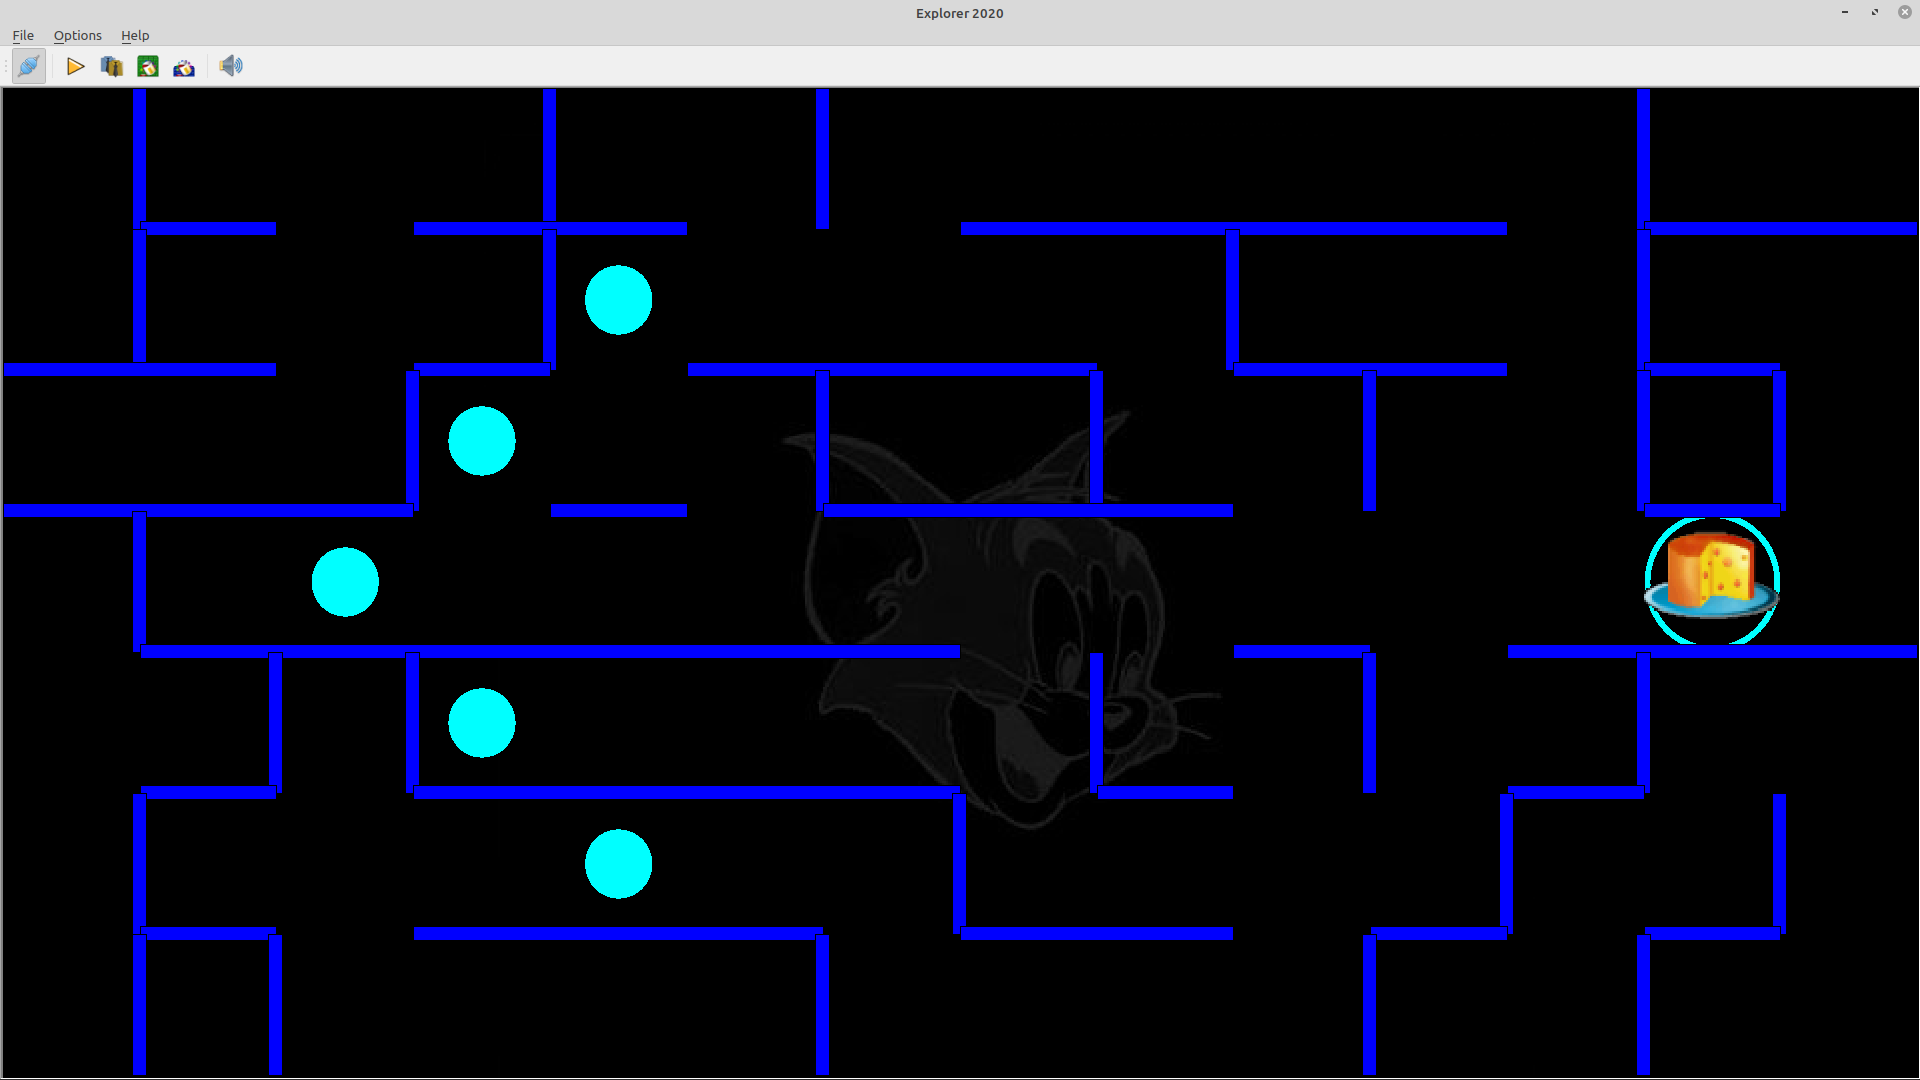
\includegraphics[width=\textwidth]{imgs/viewer_default_lab.png}
    \caption{Walls graphically displayed on the \emph{CiberRato Robot Simulation Environment}.} 
    \label{fig:map_walls_ciberrato}
\end{figure}
\FloatBarrier

\begin{figure}
    \centering
    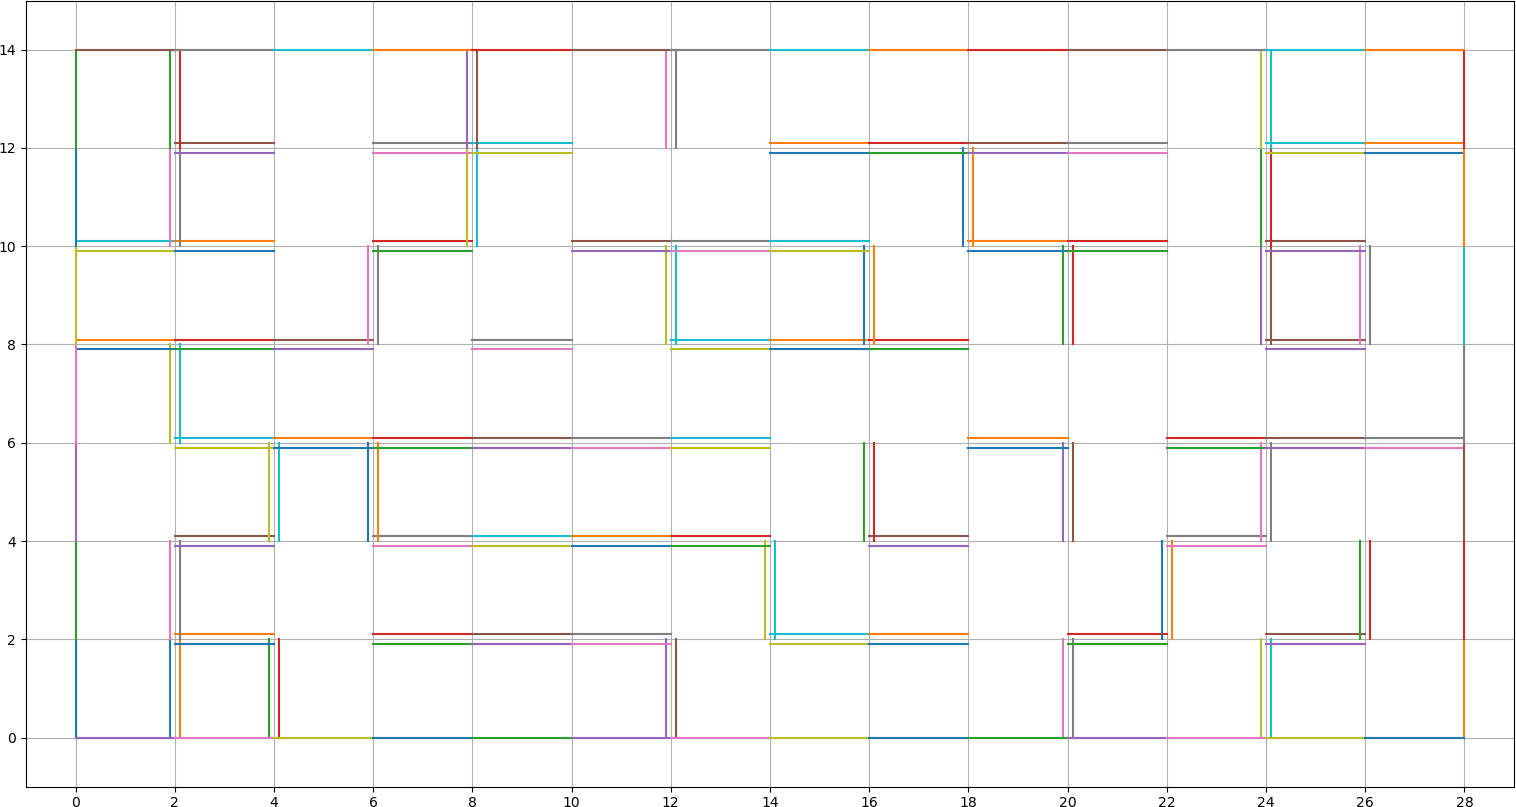
\includegraphics[width=\textwidth]{imgs/agent_walls_map.png}
    \caption{Walls graphically displayed as they are stored by the agent.} 
    \label{fig:map_walls_agent}
\end{figure}
\FloatBarrier

For the implicit outer walls that delimit the map, the coordinates are trivial to compute as they are the combination of the outer measures. 

For all the explicit inner walls, we first obtain the indices of all walls by iterating over the provided \emph{Map} structure and, then, convert the indices to the four corners, in map coordinates.

Having these coordinates, and using some geometry and vector algebra, it is possible to compute, for all sensors in all cells, the closest distance to any of the walls in the map, that lay inside the \gls{fov} of a given sensor. Notice that for this ground truth to by reliable, the sensors had to be placed in the correct position (distancing half a diameter from the center of the cell) and orientation inside each cell. On Fig. \ref{fig:walls_sensors_poses} a more visual explanation on how this was accomplished is provided.

\begin{figure}
	\centering
	\begin{subfigure}[b]{0.49\textwidth}
		\centering
		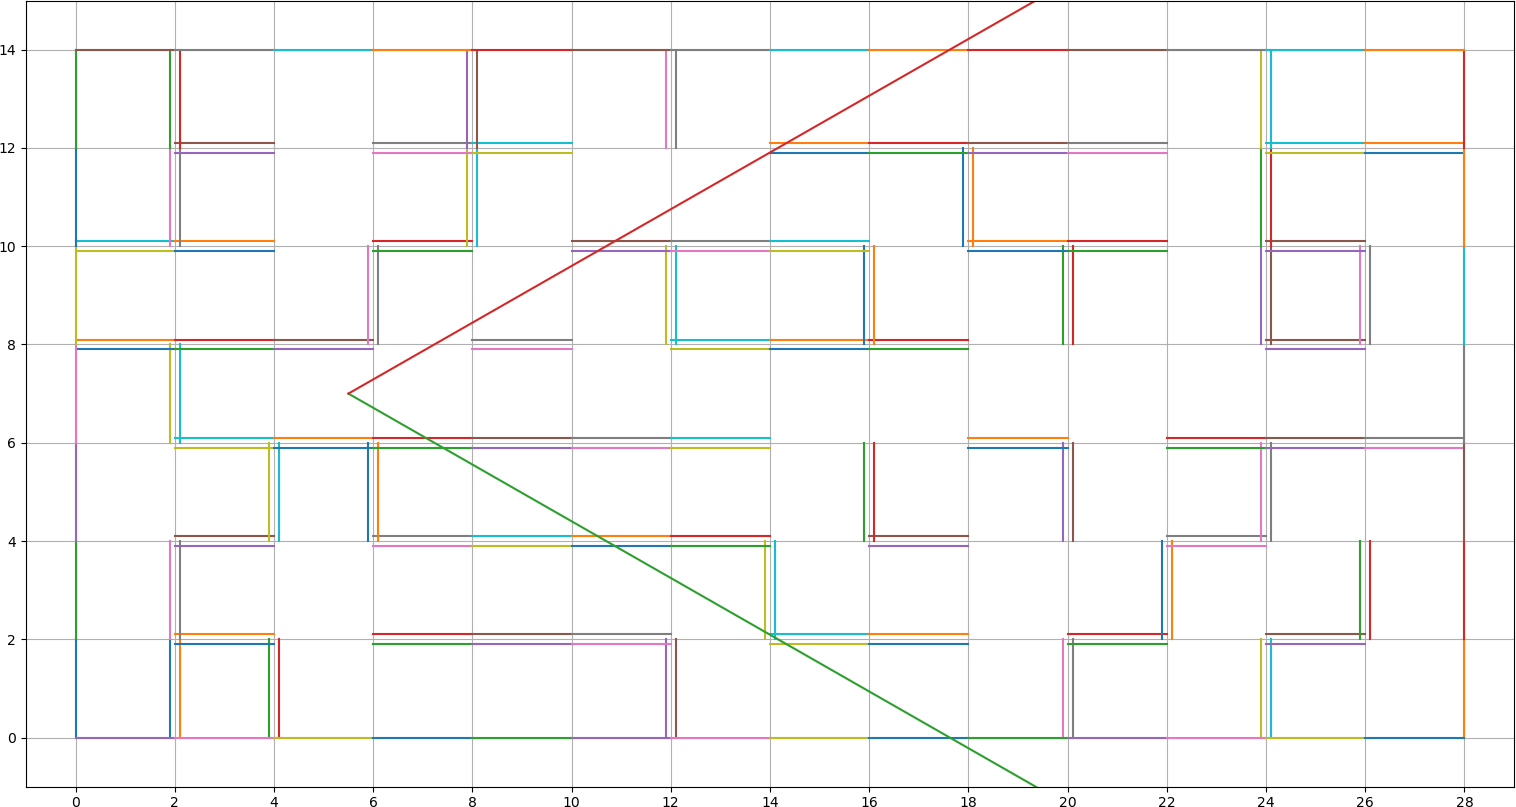
\includegraphics[width=\textwidth]{imgs/agent_map_sensor0.png}
		\caption{}
		%\label{}
	\end{subfigure}
	%
	\begin{subfigure}[b]{0.49\textwidth}
		\centering
		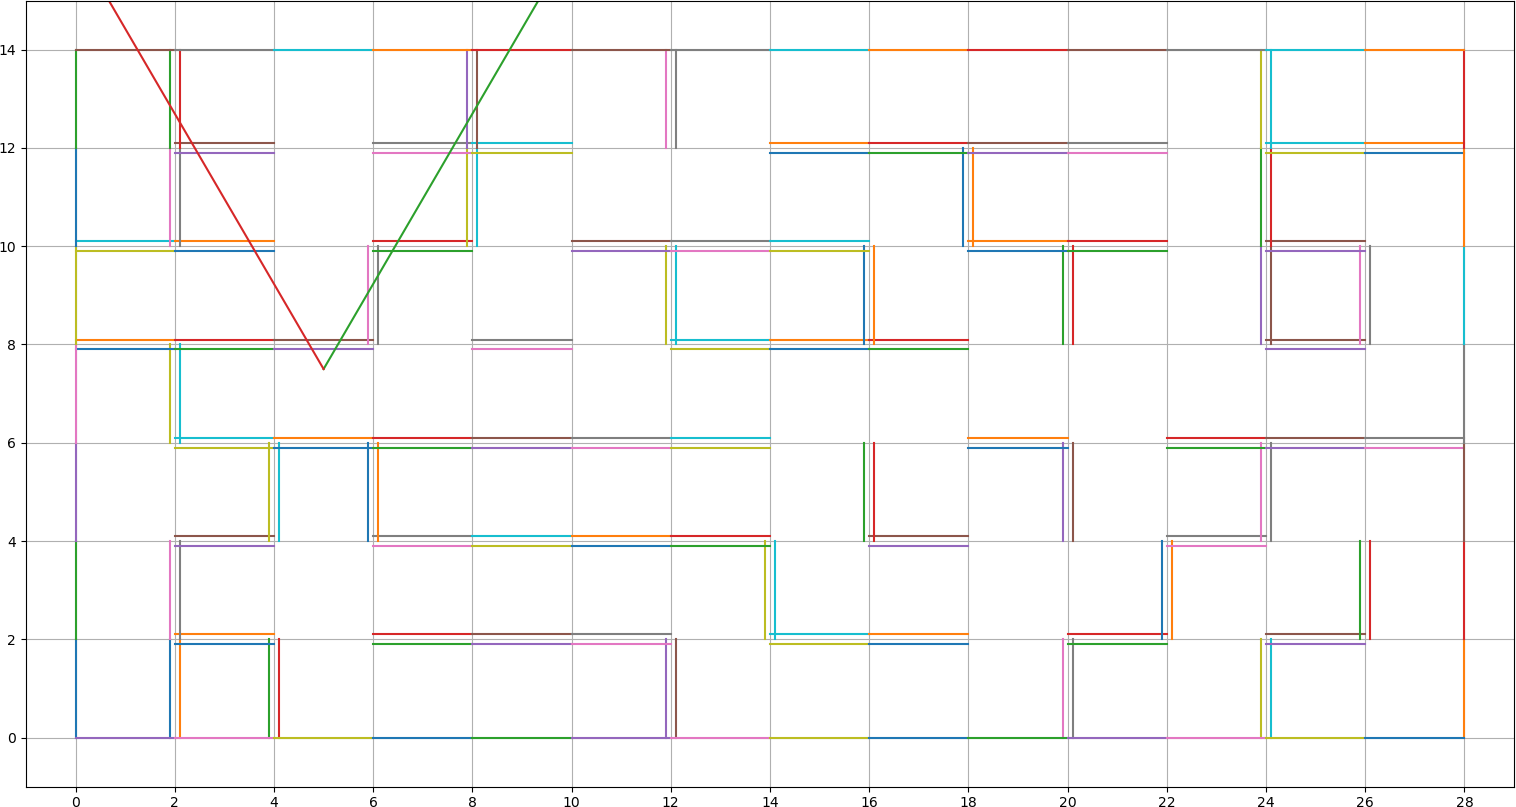
\includegraphics[width=\textwidth]{imgs/agent_map_sensor1.png}
		\caption{}
		%\label{}
	\end{subfigure}
	
	\begin{subfigure}[b]{0.49\textwidth}
		\centering
		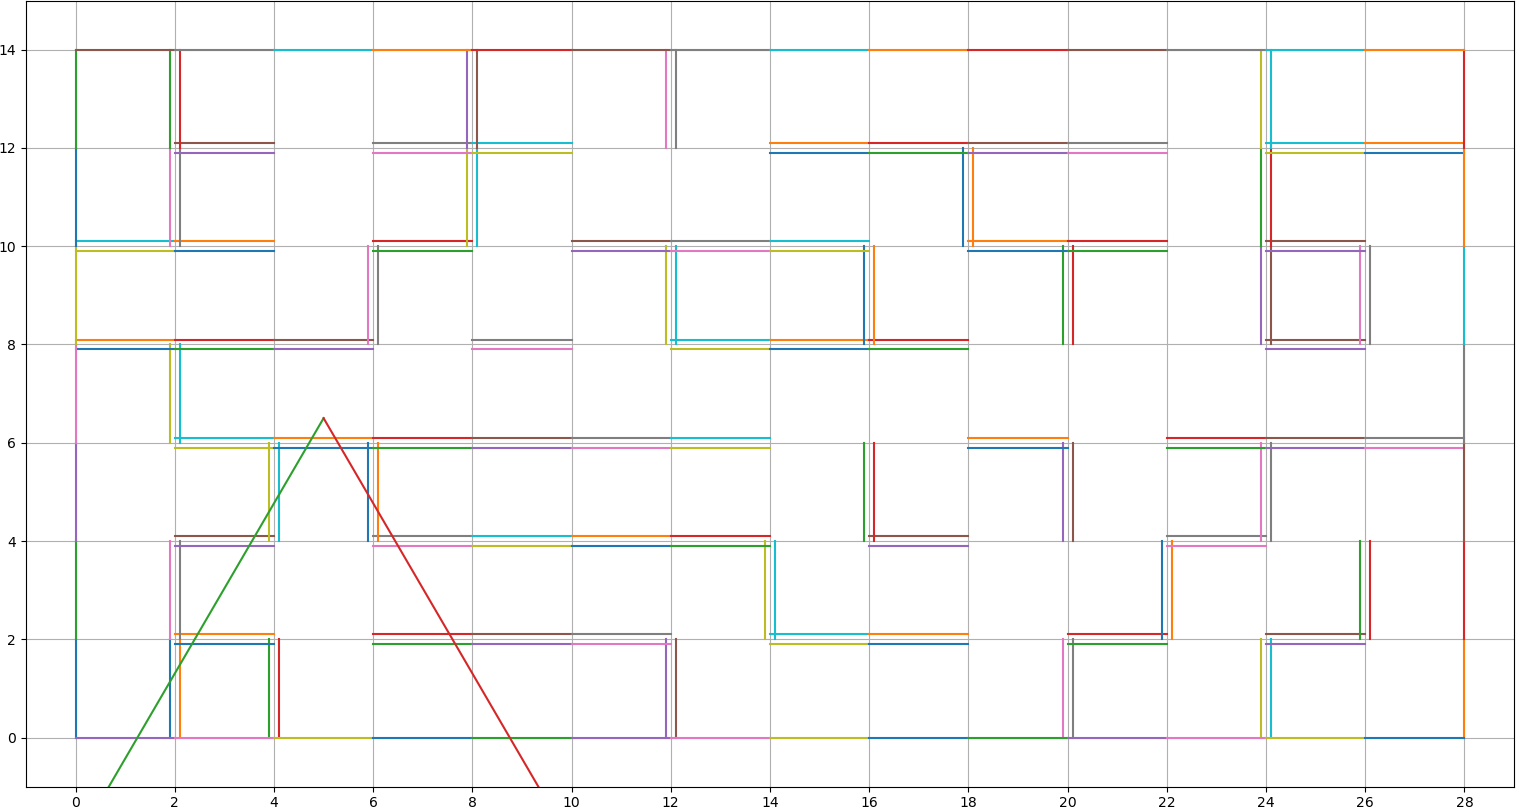
\includegraphics[width=\textwidth]{imgs/agent_map_sensor2.png}
		\caption{}
		%\label{}
	\end{subfigure}
	%
	\begin{subfigure}[b]{0.49\textwidth}
		\centering
		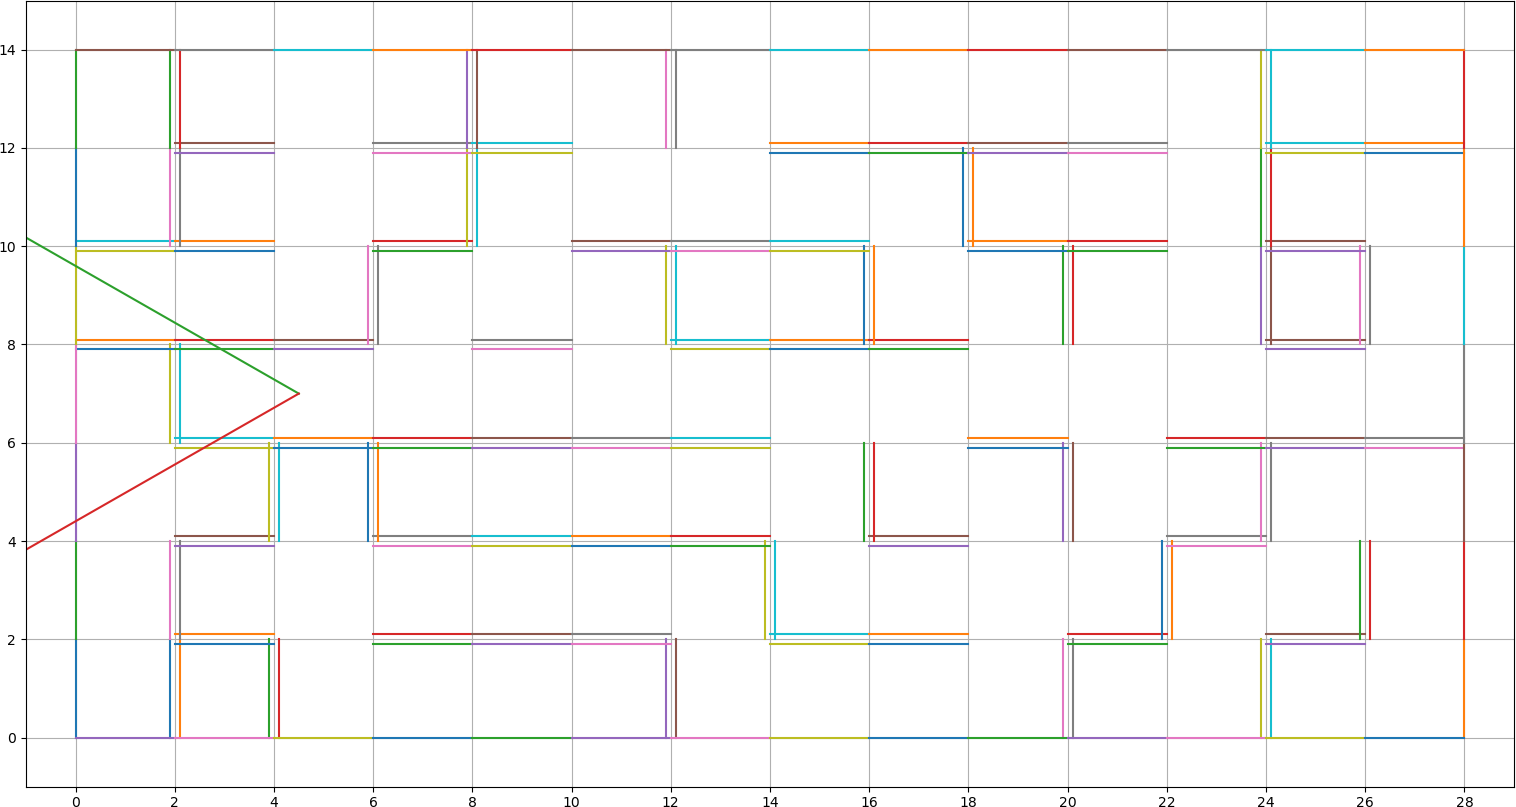
\includegraphics[width=\textwidth]{imgs/agent_map_sensor3.png}
		\caption{}
		%\label{}
	\end{subfigure}
	\caption{Sensor pose and \gls{fov} for cell (3, 2). Sensors are at (a) 0º, (b) 90º, (c) -90º and (d) 180º.}
	\label{fig:walls_sensors_poses}
\end{figure}
\FloatBarrier

\subsection{Markov Localization}
%\label{subsec:}

With the agent being in possession of the ground truth it can now start the iterative process where the initial belief is successively updated with new information (see Fig. \ref{fig:markov_flowchart}). 

\begin{figure}
    \centering
    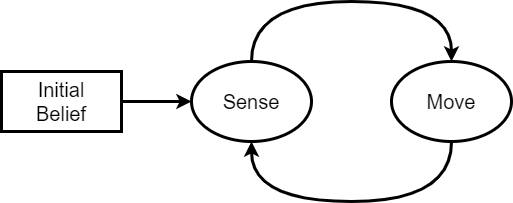
\includegraphics[width=\textwidth]{imgs/flowchart.png}
    \caption{Flowchart of the iterative localization procedure (Markov localization).} 
    \label{fig:markov_flowchart}
\end{figure}
\FloatBarrier

The agent is continually updating its displacement since the staring of the simulation up until the present moment. This is necessary so that the agent knows when it has arrived to a new cell (actually, the center of the cell). The agent does, in fact, know how much it has moved because the noise on the motors is null. If it was not, this would only be a prediction. 

At the start of the simulation, the robot is stationary and, so, the displacement is null. The agent will use this control action to update the initial belief but, as demonstrated on section \ref{subsec:bayes_filter}, when $u_t = [0, 0]$ there are no changes in the probabilities distribution.

Immediately after this, the \gls{ir} sensors measures are integrated using algorithm \ref{alg:bayes_sense} and the agent waits until it reaches a new cell to iterate the process again. This time, given that the motion was not null ($u_t = [1, 0]$) the Motion Update will cause a shift on the probability distribution.

\subsection{Known Limitations}
%\label{subsec:debug_tools}

There are some known limitations in the present work. These are stated bellow:

\begin{enumerate}
    \item The Motion Update procedure is only developed for stationary or one cell right motion control actions. This is on purpose because i) other motions are outside the scope of this assignment and ii) it limits the amount of code needed to compute the updated belief.
    \item The computation of the ground truth is relatively slow. Because of this, the algorithm runs on another \emph{thread} and the actual updating of the beliefs, at each time step, is only done after the simulation ended (\emph{offline} approach). At this stage, the agent should have finish gathering the measurements and control actions at each cell of the simulation.
    \item The agent uses the collision detection has a termination criteria. This works well is the scope of this assignment given the single \gls{dof} of the motion, but would be counterproductive in a real world scenario.
\end{enumerate}

\section{Results}
\label{sec:results}

On Fig. \ref{fig:localization_example}, a demonstration of the localization process is presented. At the starting state (Fig. \ref{fig:localization_step0}) the agent is completely unaware of its position on the map (again using the same map as on section \ref{subsec:ground_truth} for an easier understanding). Then, as it senses the surroundings and moves, both for the first time, the pool of possible locations shrinks (see Fig. \ref{fig:localization_step1}), becoming just two possibilities with equal chances within the next two iterations (see Figs. \ref{fig:localization_step2} and \ref{fig:localization_step3}). In posterior evaluations, the agent is completely sure of its position (see trough Figs. \ref{fig:localization_step4} to \ref{fig:localization_step12}) \footnote{Video available on \url{https://youtu.be/gf-PzjpjPEI}}.

\begin{figure}
	\centering
	\begin{subfigure}[b]{0.32\textwidth}
		\centering
		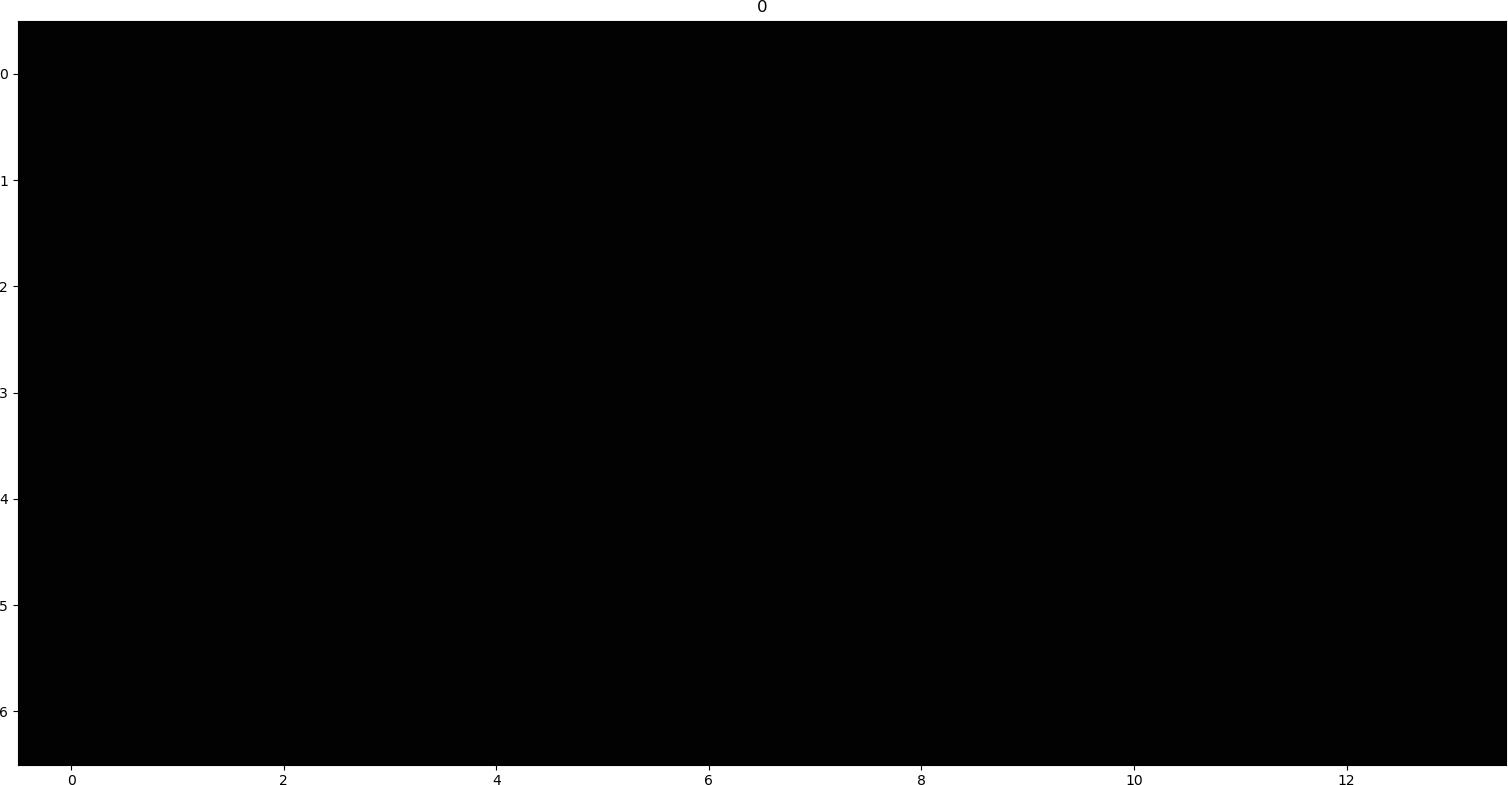
\includegraphics[width=\textwidth]{imgs/prediction_default_lab/it_00.png}
		\caption{}
		\label{fig:localization_step0}
	\end{subfigure}
	%
	\begin{subfigure}[b]{0.32\textwidth}
		\centering
		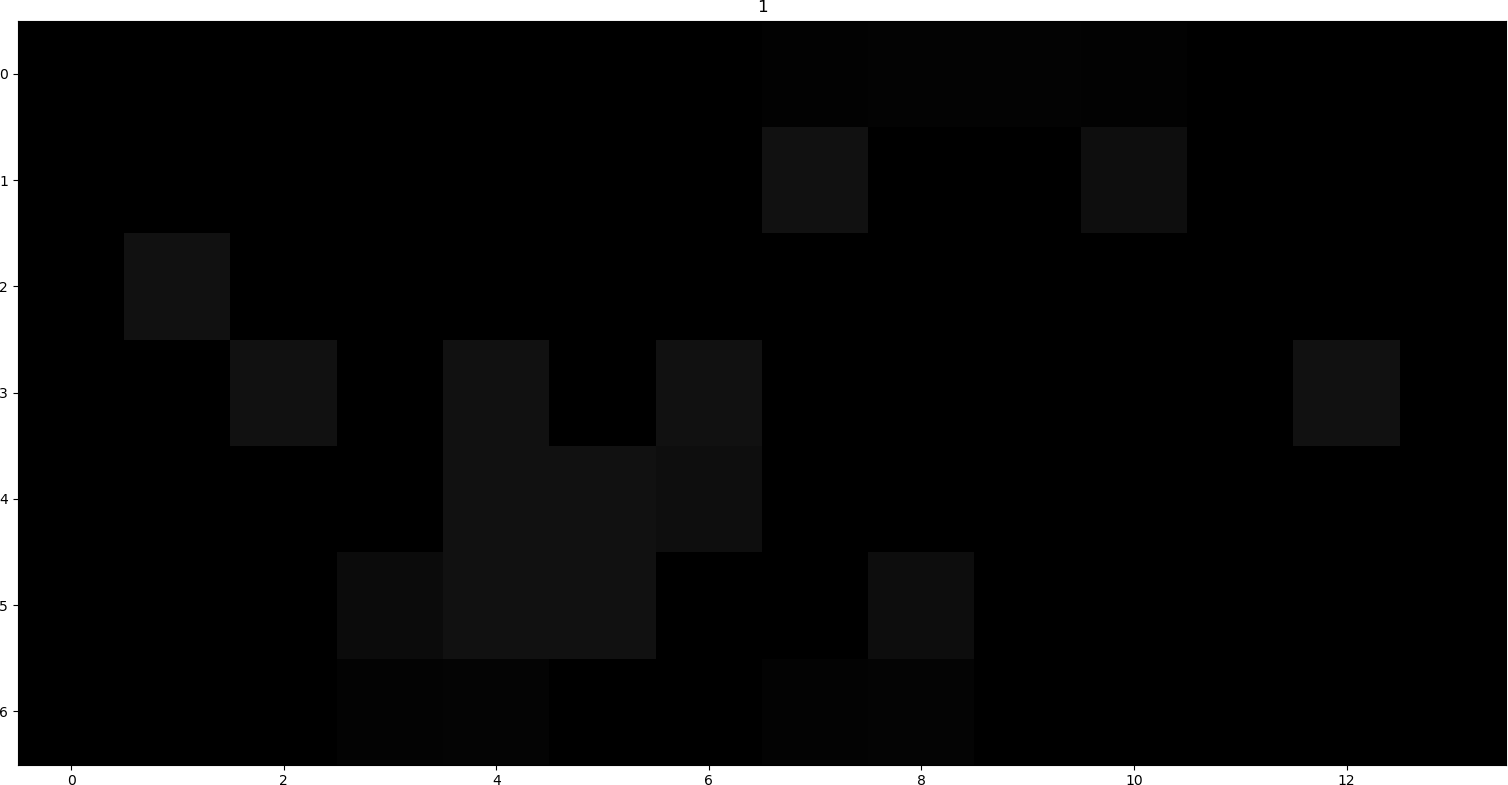
\includegraphics[width=\textwidth]{imgs/prediction_default_lab/it_01.png}
		\caption{}
		\label{fig:localization_step1}
	\end{subfigure}
	%
	\begin{subfigure}[b]{0.32\textwidth}
		\centering
		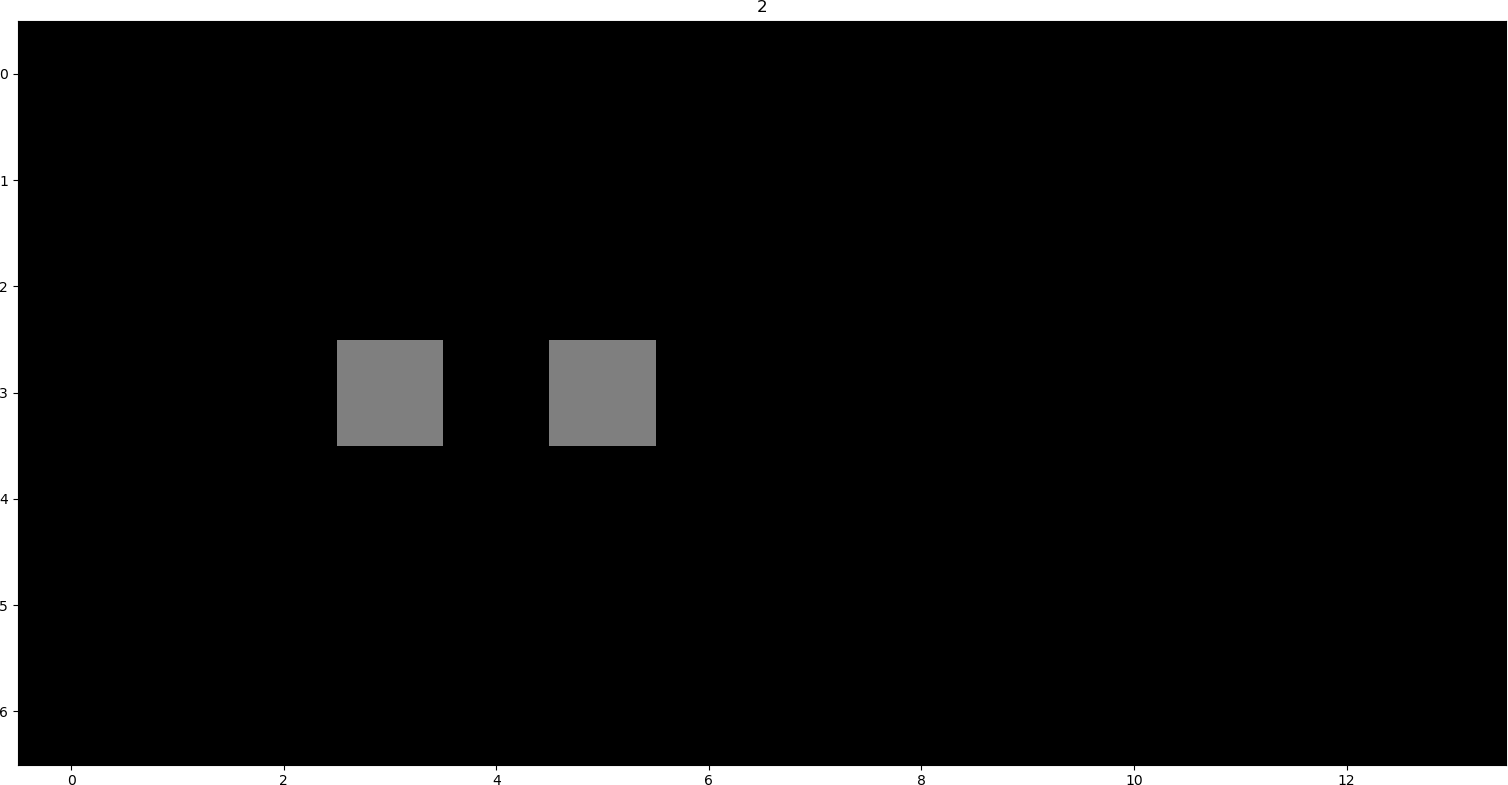
\includegraphics[width=\textwidth]{imgs/prediction_default_lab/it_02.png}
		\caption{}
		\label{fig:localization_step2}
	\end{subfigure}
	
	\begin{subfigure}[b]{0.32\textwidth}
		\centering
		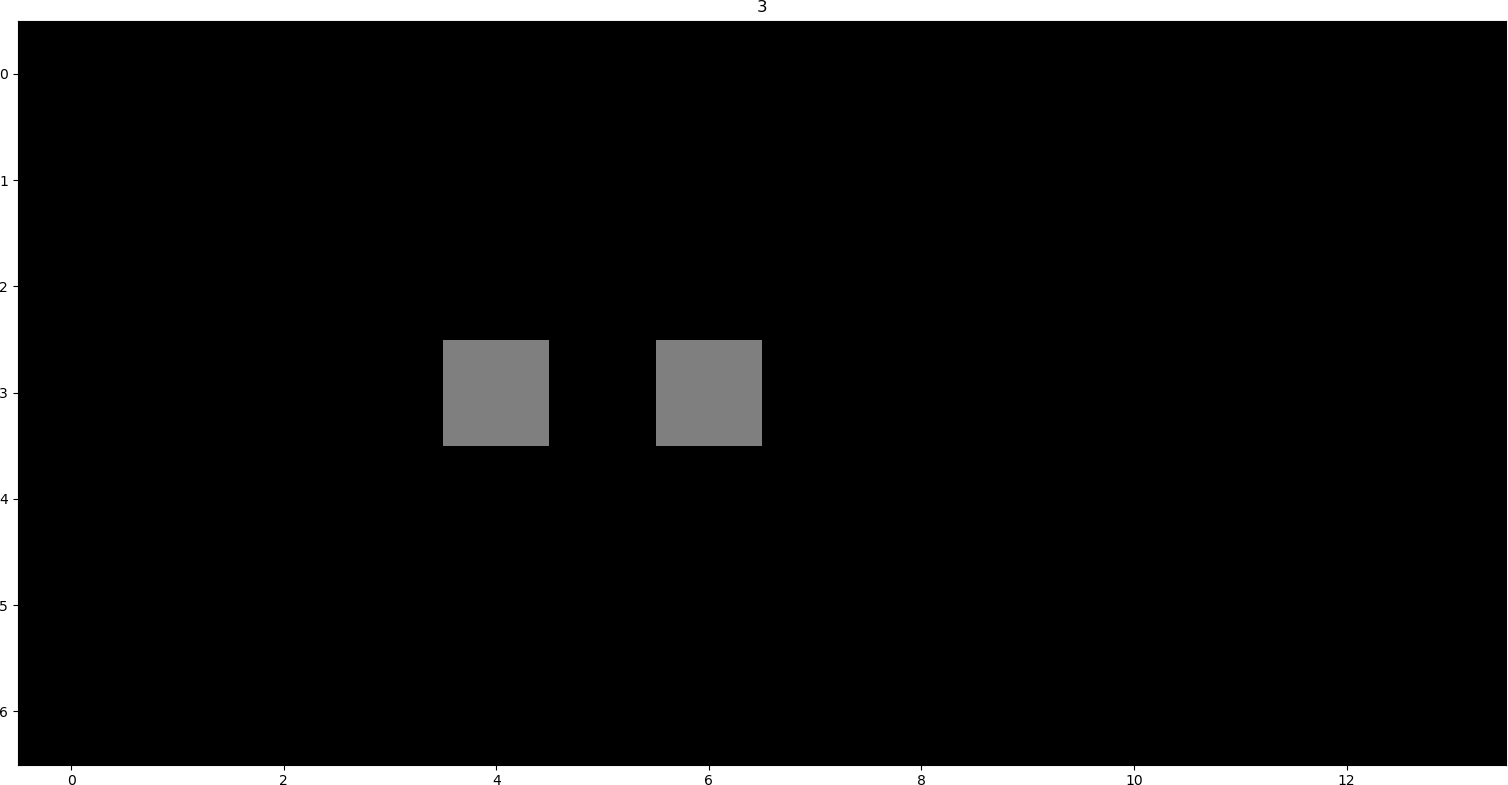
\includegraphics[width=\textwidth]{imgs/prediction_default_lab/it_03.png}
		\caption{}
		\label{fig:localization_step3}
	\end{subfigure}
	%
	\begin{subfigure}[b]{0.32\textwidth}
		\centering
		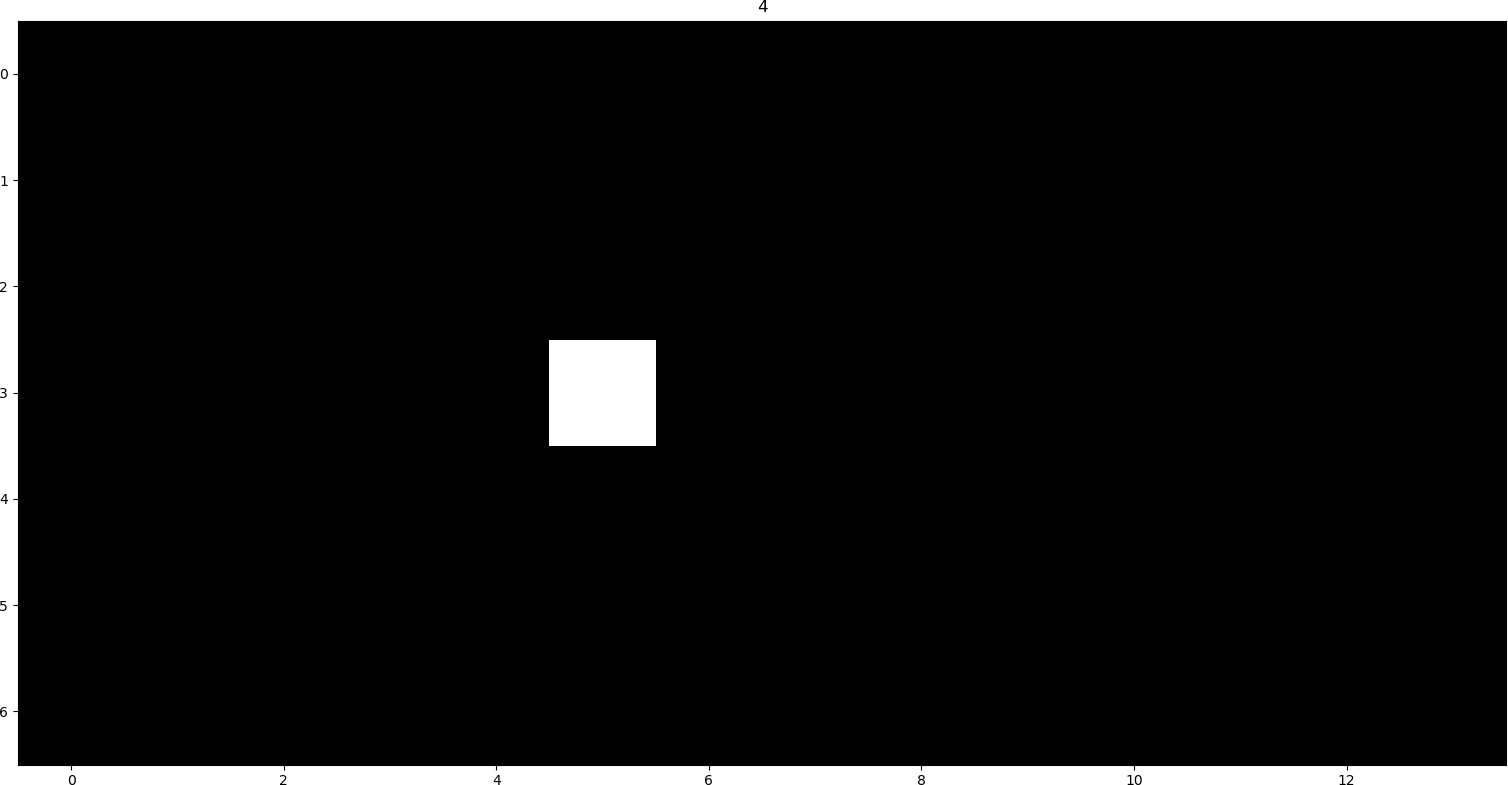
\includegraphics[width=\textwidth]{imgs/prediction_default_lab/it_04.png}
		\caption{}
		\label{fig:localization_step4}
	\end{subfigure}
	%
	\begin{subfigure}[b]{0.32\textwidth}
		\centering
		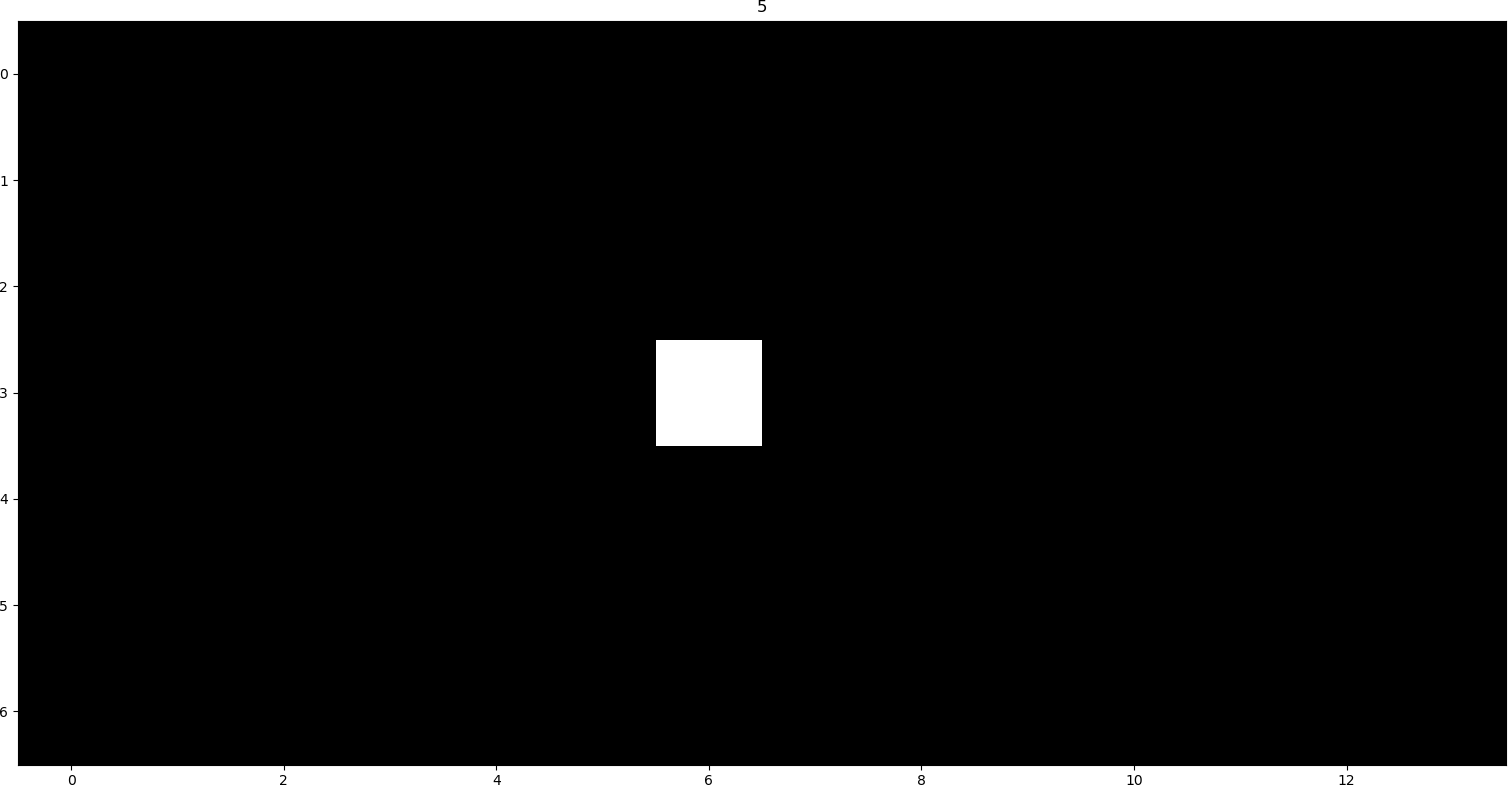
\includegraphics[width=\textwidth]{imgs/prediction_default_lab/it_05.png}
		\caption{}
		\label{fig:localization_step5}
	\end{subfigure}
	
	\begin{subfigure}[b]{0.32\textwidth}
		\centering
		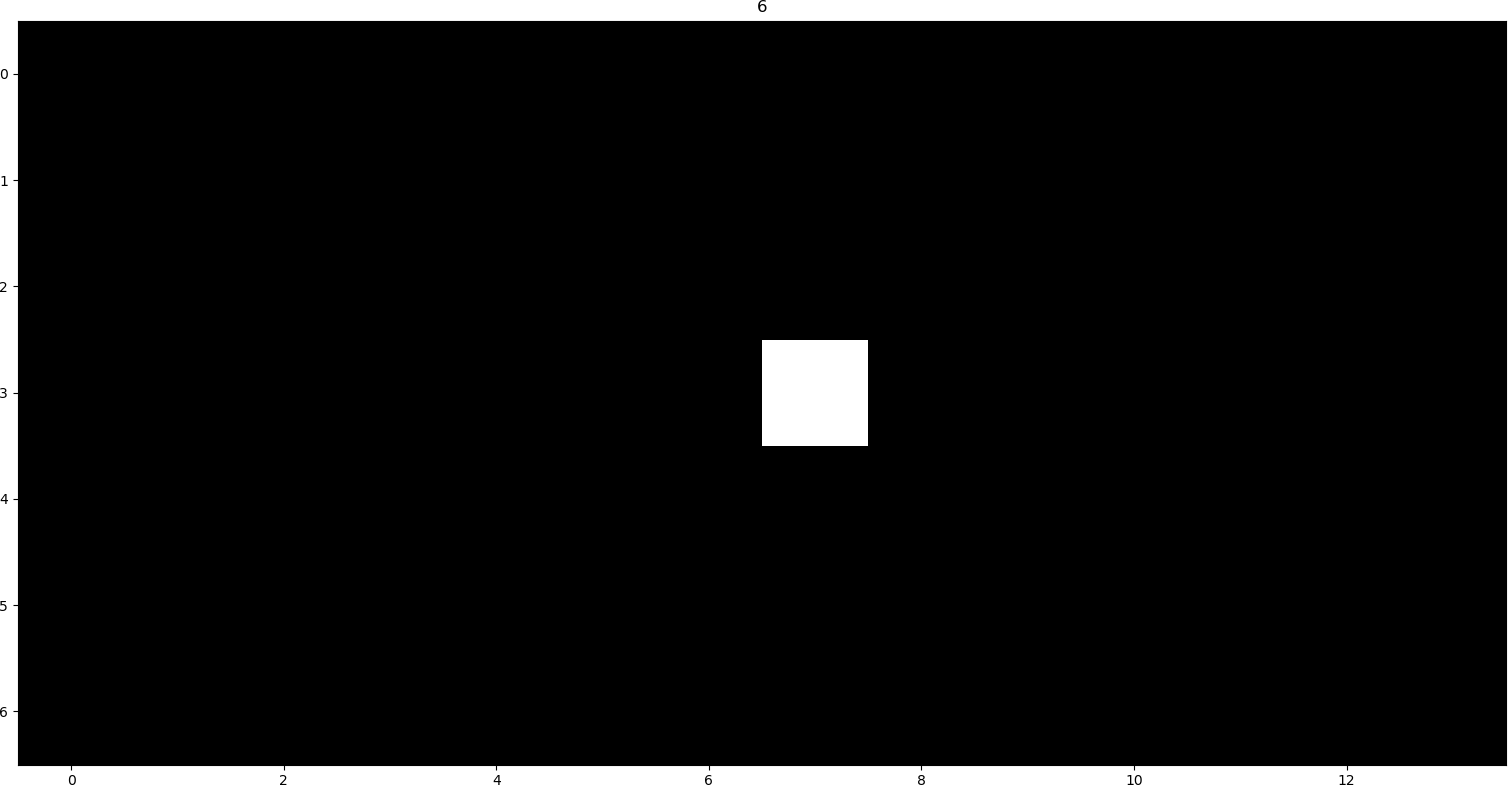
\includegraphics[width=\textwidth]{imgs/prediction_default_lab/it_06.png}
		\caption{}
		\label{fig:localization_step6}
	\end{subfigure}
	%
	\begin{subfigure}[b]{0.32\textwidth}
		\centering
		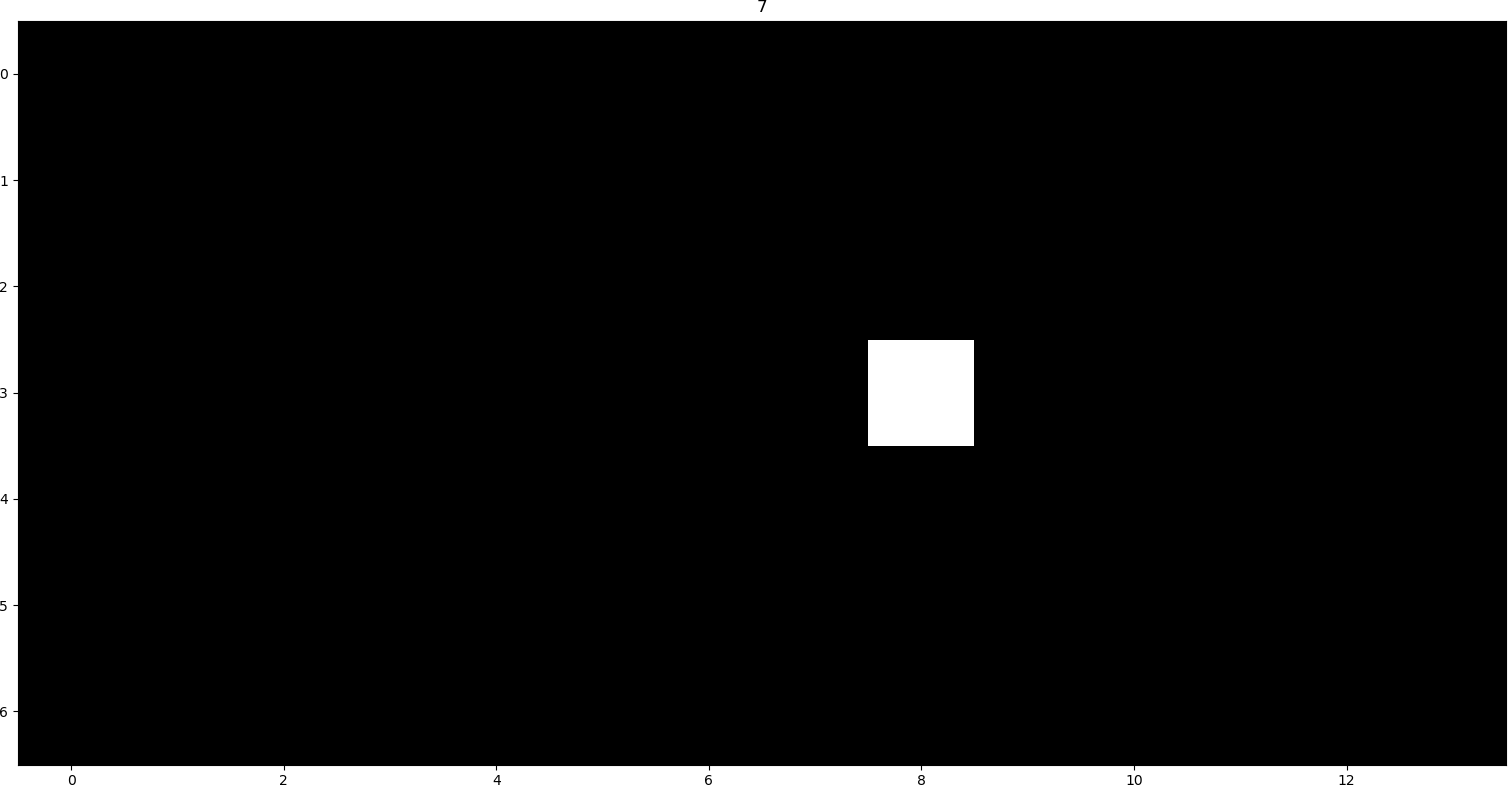
\includegraphics[width=\textwidth]{imgs/prediction_default_lab/it_07.png}
		\caption{}
		\label{fig:localization_step7}
	\end{subfigure}
	%
	\begin{subfigure}[b]{0.32\textwidth}
		\centering
		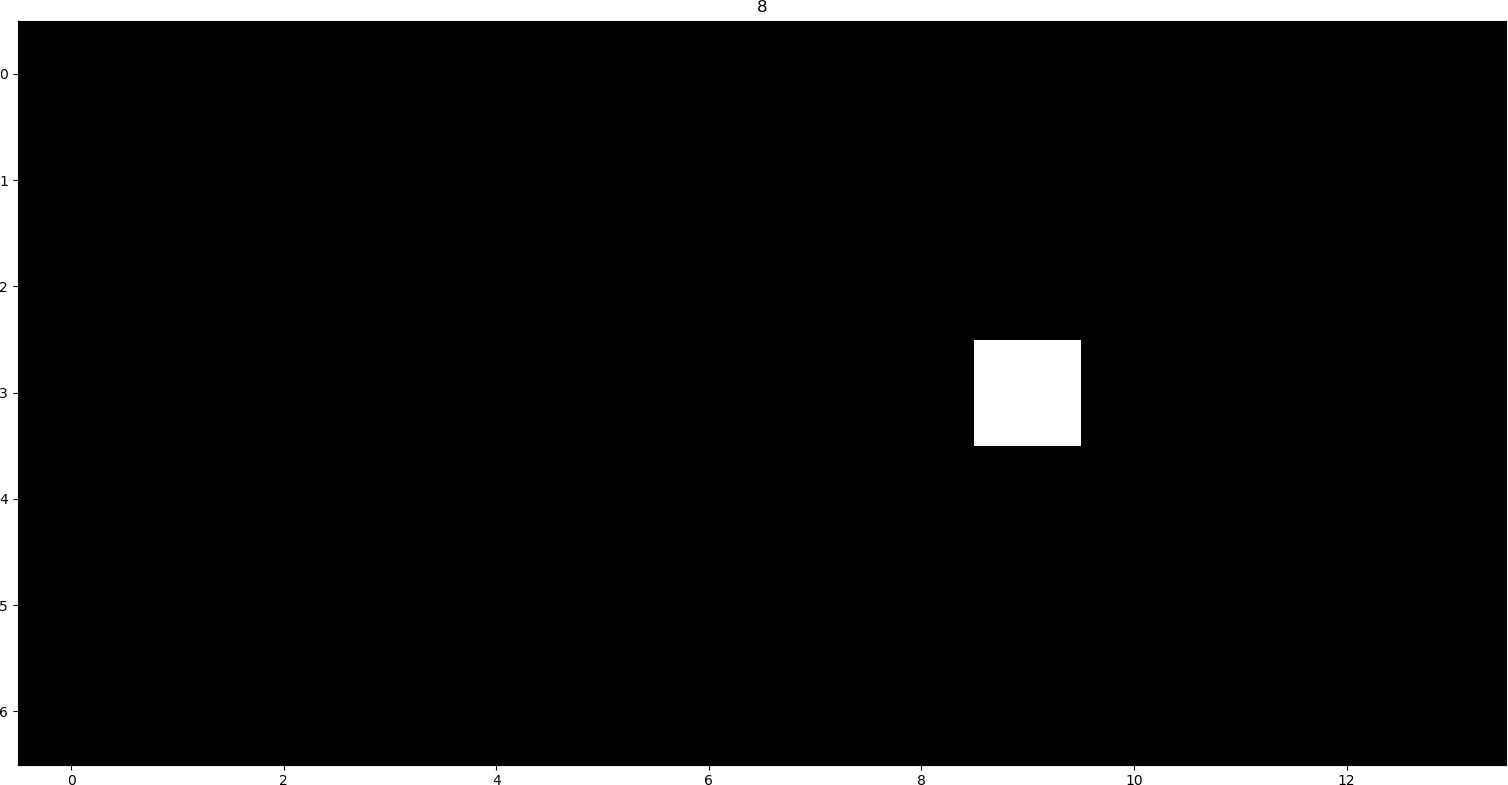
\includegraphics[width=\textwidth]{imgs/prediction_default_lab/it_08.png}
		\caption{}
		\label{fig:localization_step8}
	\end{subfigure}
	
	\begin{subfigure}[b]{0.32\textwidth}
		\centering
		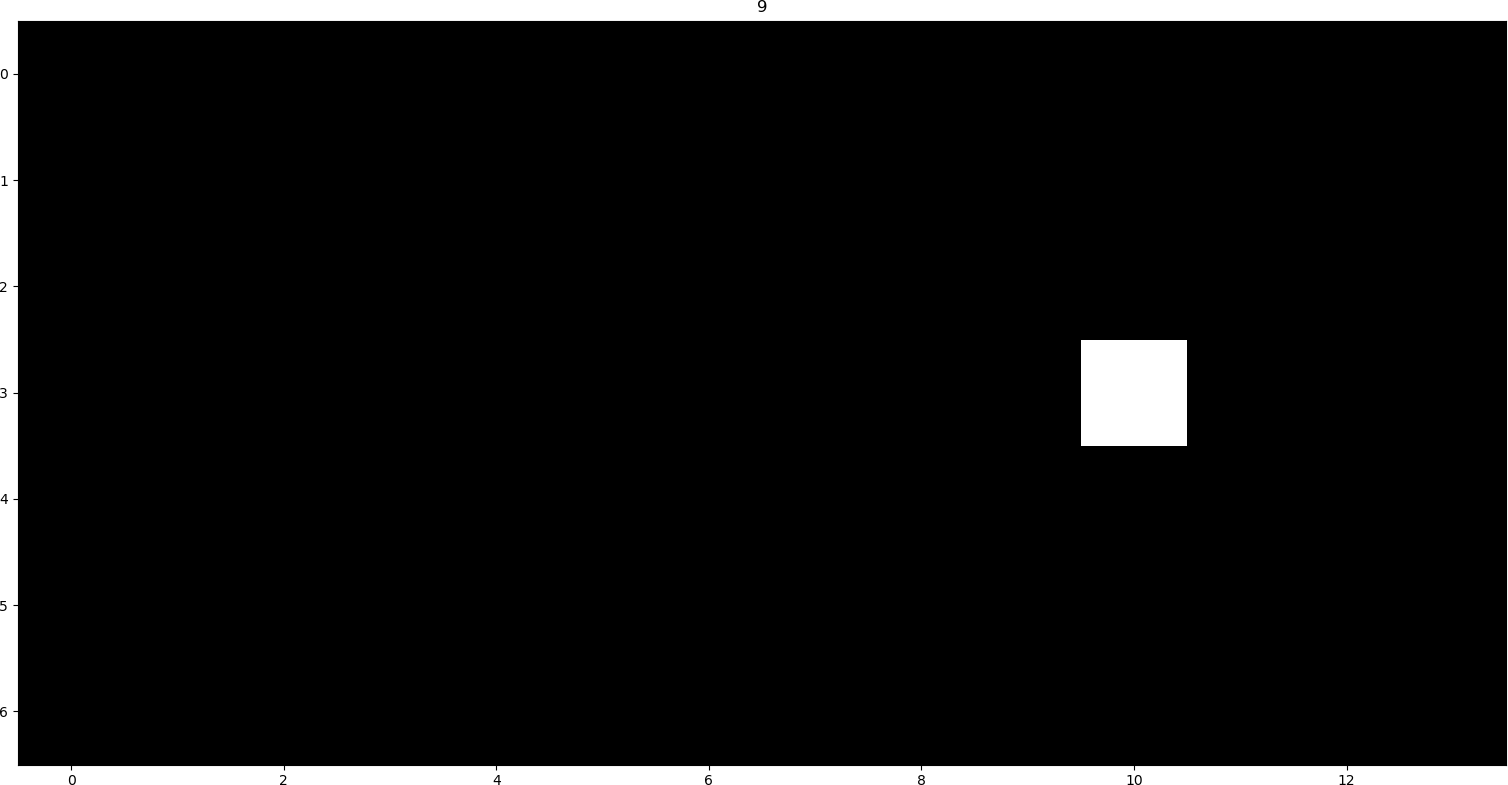
\includegraphics[width=\textwidth]{imgs/prediction_default_lab/it_09.png}
		\caption{}
		\label{fig:localization_step9}
	\end{subfigure}
	%
	\begin{subfigure}[b]{0.32\textwidth}
		\centering
		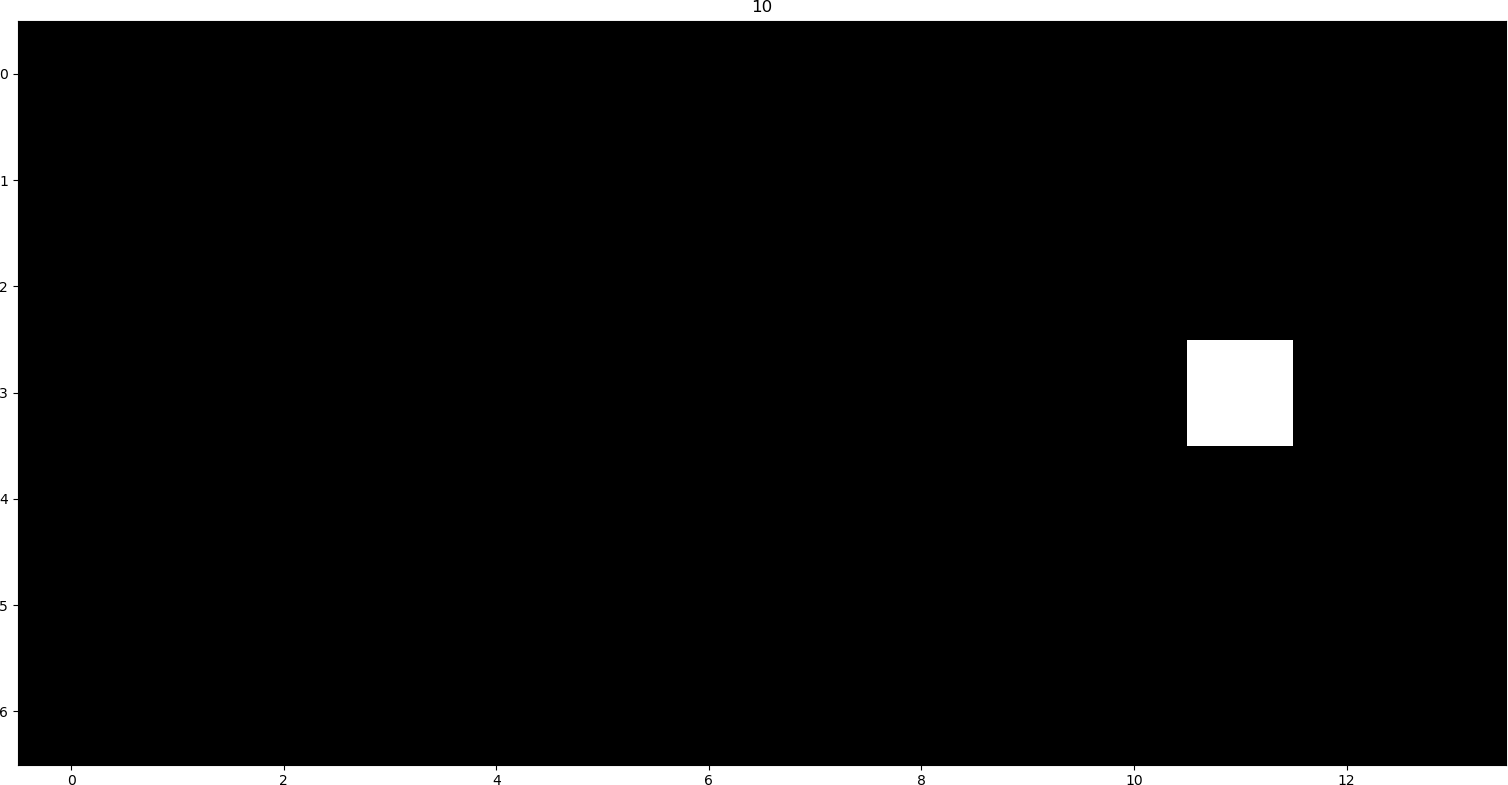
\includegraphics[width=\textwidth]{imgs/prediction_default_lab/it_10.png}
		\caption{}
		\label{fig:localization_step10}
	\end{subfigure}
	%
	\begin{subfigure}[b]{0.32\textwidth}
		\centering
		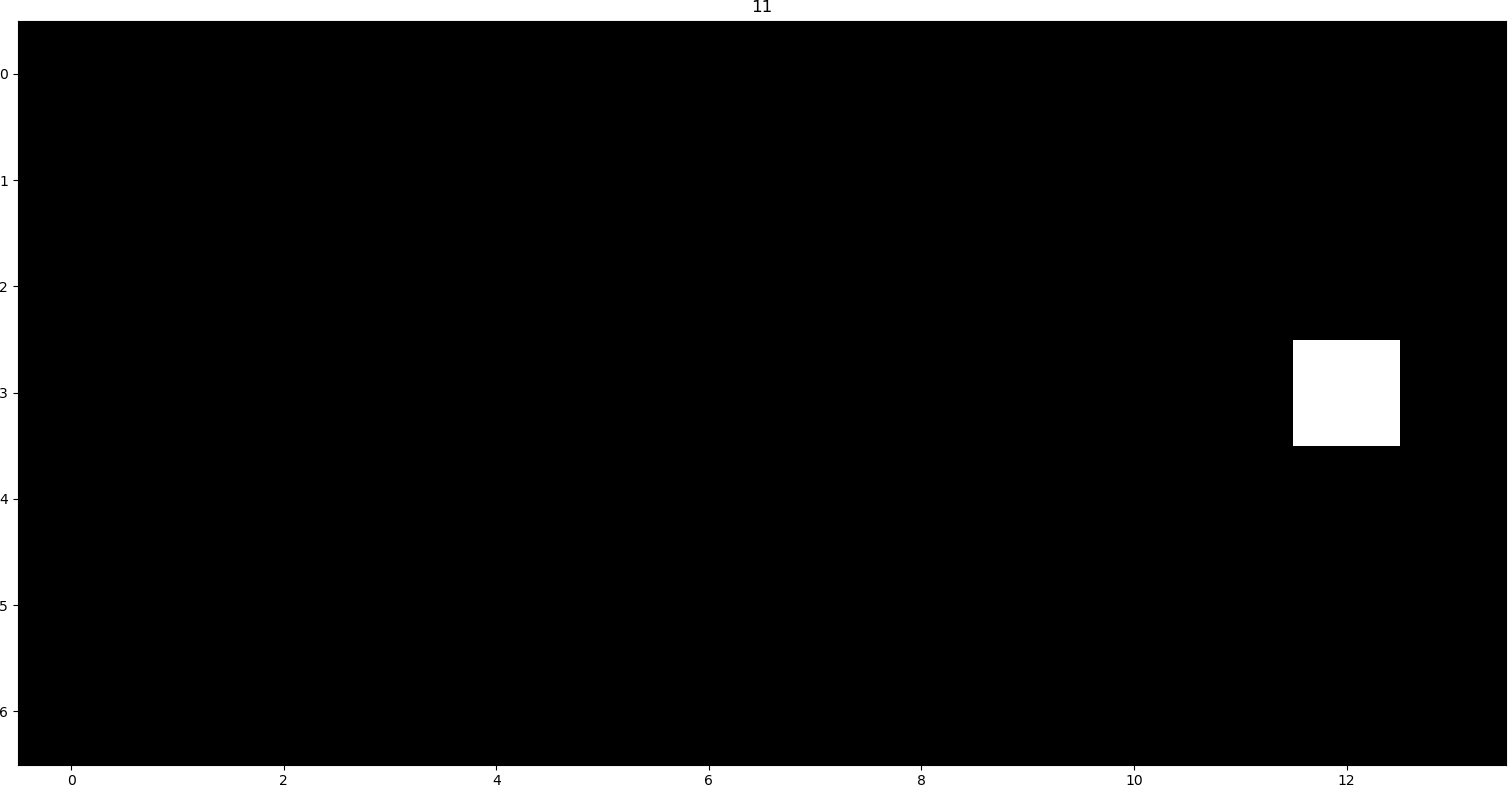
\includegraphics[width=\textwidth]{imgs/prediction_default_lab/it_11.png}
		\caption{}
		\label{fig:localization_step11}
	\end{subfigure}
	
	\begin{subfigure}[b]{0.32\textwidth}
		\centering
		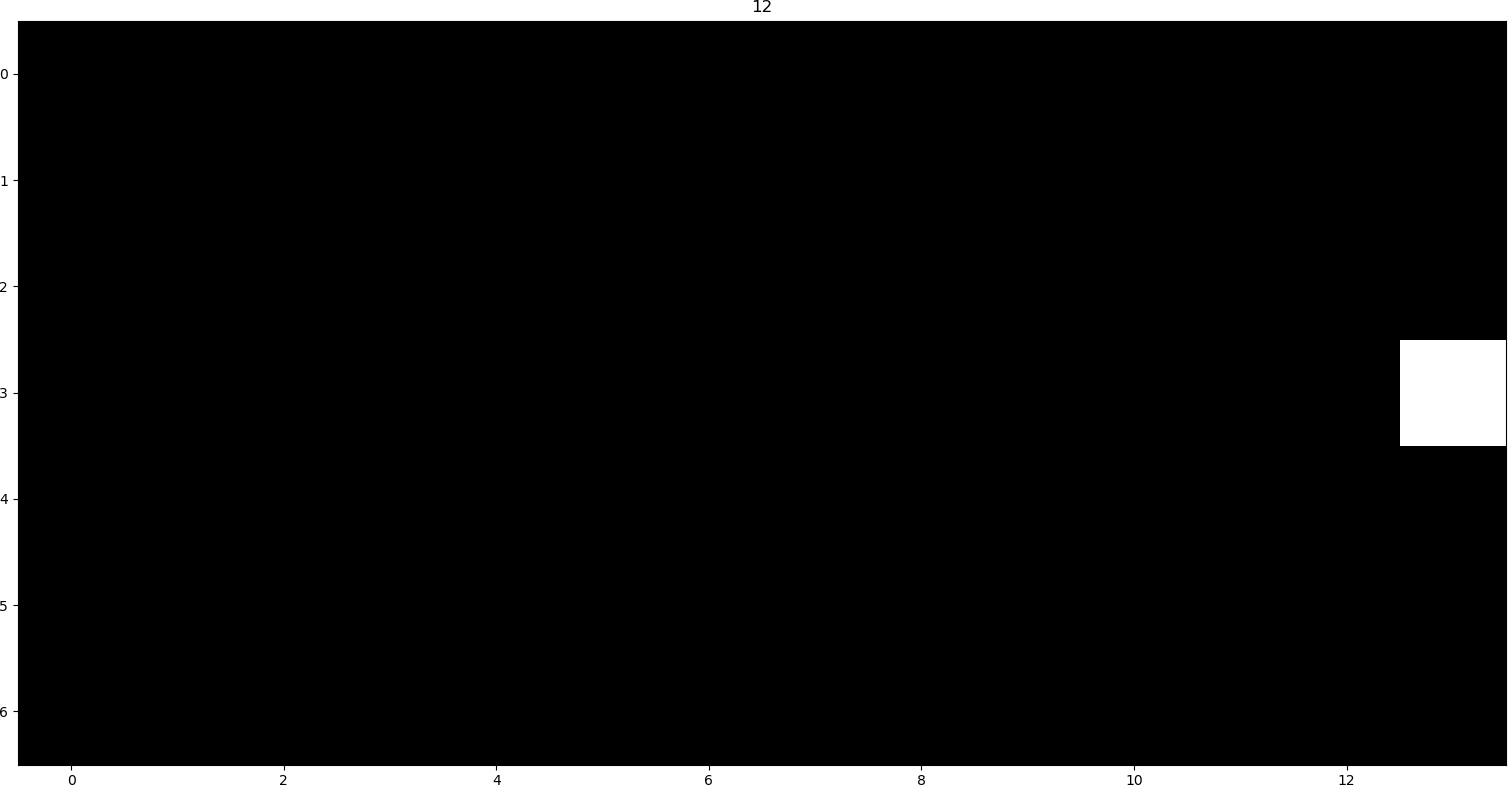
\includegraphics[width=\textwidth]{imgs/prediction_default_lab/it_12.png}
		\caption{}
		\label{fig:localization_step12}
	\end{subfigure}
	%
	\caption{Visual representation of the agent localization belief updating process.}
	\label{fig:localization_example}
\end{figure}
\FloatBarrier





%
% ---- Bibliography ----
%
% BibTeX users should specify bibliography style 'splncs04'.
% References will then be sorted and formatted in the correct style.
%
\bibliographystyle{splncs04}
\bibliography{bib}
%
\end{document}
